\documentclass{beamer}
%\documentclass[aspectratio=169]{beamer}
%
\mode<presentation>
{
  \usetheme{default}      
  \usecolortheme{default}
  \usefonttheme{default} 
  \setbeamertemplate{navigation symbols}{}
  \setbeamertemplate{caption}[numbered]
} 

\usepackage[english]{babel}
\usepackage[utf8x]{inputenc}
\usepackage{bbm}

\newcommand{\1}[1]{\mathbbm{1}\left[#1\right]}
\newcommand{\norm}[1]{\left\lVert#1\right\rVert}

\title[Classification]{Introduction to Machine Learning}
\subtitle{Lecture 5: Model Selection and Validation}
\author{Alexis Zubiolo\newline\texttt{alexis.zubiolo@gmail.com}}
\institute{Data Science Team Lead @ Adcash}
\date{\today}

\begin{document}

\begin{frame}
  \titlepage
\end{frame}

\begin{frame}
\textbf{Shameless advertisement}: There will be a more advanced course starting in January 2017!
\vfill
More info:
\begin{center}
http://itstep.bg/news-bg/kurs-machine-learning-from-scratch/
\end{center}
\end{frame}

\begin{frame}{Introduction}
Model evaluation is a key component of a machine learning pipeline.
\pause
\vfill
It makes it possible to chose a set of hyper-parameters so that
\begin{itemize}
	\item The model is accurate enough
	\item The model generalizes well (\textit{i.e.} does not over-fit)
\end{itemize}
\vfill
\pause
Recall from lecture 3:
\begin{figure}
\centering
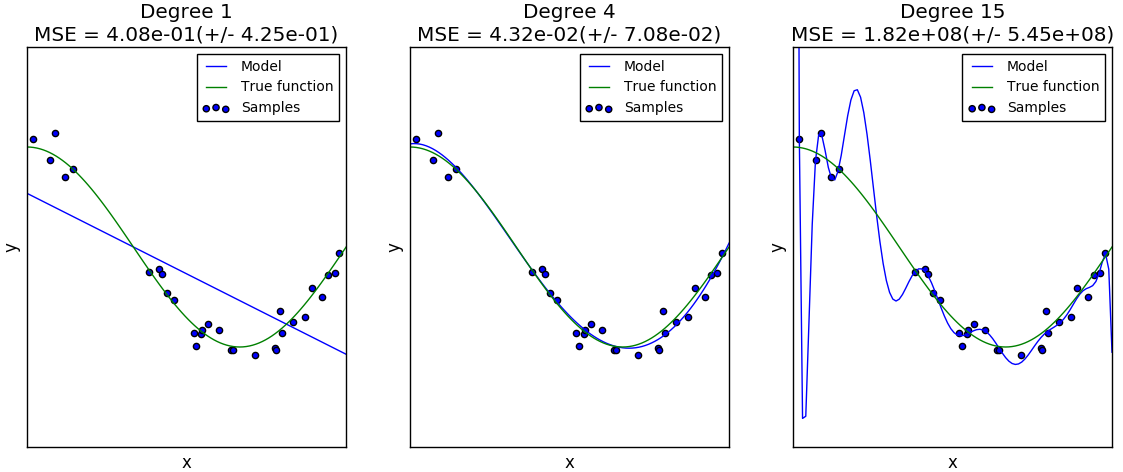
\includegraphics[width=\textwidth]{images/over_under_fitting.png}
\end{figure}
\end{frame}

\begin{frame}
Course outline:
\begin{itemize}
	\item Evaluation metrics, what they mean
	\item How/when/why yo apply them
\end{itemize}
\end{frame}

\begin{frame}
\begin{center}
\Huge{Evaluation metrics}
\end{center}
\end{frame}

\begin{frame}{Accuracy}

\end{frame}

\begin{frame}{Confusion matrix}

\end{frame}

\begin{frame}{Machine learning loss}
0-1 loss:
$$ \ell \left( \hat{y}, y \right) = \1{\hat{y} = y}$$
\vfill
\pause
Squared loss:
$$ \ell \left( \hat{y}, y \right) = \left( \hat{y} - y\right)^2$$
\vfill
\pause
Hinge loss:

\vfill
\pause
Squared hinge loss:

\vfill
\pause
Log-loss:
\vfill
\pause
Possibility to add a weight the loss!

\end{frame}

\begin{frame}{Precision, recall}

\end{frame}

\begin{frame}{ROC curve}

\end{frame}

\begin{frame}
\begin{center}
\Huge{Applying evaluation metrics}
\end{center}
\end{frame}

\begin{frame}{Train-test split}
Reminder: ML algorithms (classification/regression) often rely on \textbf{many parameters}. How to \textbf{tune} them properly given a data set?
\vfill
\pause
The most commonly used principle is the train-test split:
\begin{itemize}
	\item \textbf{Split the data} into a training set and a test set
	\item \textbf{Train} on the training set
	\item \textbf{Test} on the test set
\end{itemize}
\vfill
\pause
This is often referred to as \textbf{cross-validation}.
\end{frame}

\begin{frame}{Cross-validation}
Standard technique: $k$-fold cross-validation
\begin{itemize}
	\item Split the data into $k$ equally sized folds
	\item Remove 1 fold (= test fold)
	\item Train on the other folds
	\item Test on the removed fold
	\item Do it for all the folds
\end{itemize}
\vfill
\pause
Note: It is often advised to perform a \textbf{stratified} cross-validation, \textit{i.e.} each fold contains approximately the \textbf{same percentage} of samples of each target class \textbf{as the complete set}.
\end{frame}

\begin{frame}{Small data set}
Suppose you have \textbf{a small data set}. How to evaluate a classifier in this case?
\vfill
\pause
$k$-fold cross-validation? Even with $k = 2$, it would make the training set even smaller and make it hard to fit a proper model.
\vfill
\pause
Other option: \textbf{Leave-one-out} (LOO) cross-validation:
\pause
\begin{itemize}
	\item \textbf{Remove 1 sample} from the data set
	\item Train on \textbf{all the other samples}
	\item Test on the sample you've removed
	\item \textbf{Evaluate} the prediction
	\item Do it \textbf{for each sample of the data set}
	\item \textbf{Aggregate} the evaluations
\end{itemize}
\pause
\vfill
\textbf{Remark}: This could lead to many iterations even if the data set is small.
\pause
\vfill
\textbf{Alternative}: Leave-$p$-out (LPO)
\end{frame}

\begin{frame}{Parameter selection}
One of the goals of model evaluation is to select a \textbf{good model}.
\vfill
\pause
Hence we want to choose one (or several) hyper-parameters. How do we do?
\vfill
\pause
Most classic way: a \textbf{grid-search}
\begin{itemize}
	\item For each parameter, define a set of possible values
	\item For each parameter combination, train/test the model
	\item Pick the parameter combination which gives best results
\end{itemize}
\vfill
\pause
\textbf{Example}: SVM with kernel degree $\in \{1, 2, 3, 4, 5\}$ and soft-margin parameter $\in \{0.01, 0.1, 1, 10 \}$.
\vfill
\pause
\textbf{Important note}: Hyper-parameter ranges vary a lot from an application to another. It is \textbf{data-dependent}.
\end{frame}

\begin{frame}{Grid search vs random search}
Random search is a more and more popular alternative to grid search:
\vfill
\pause
\begin{figure}
\centering
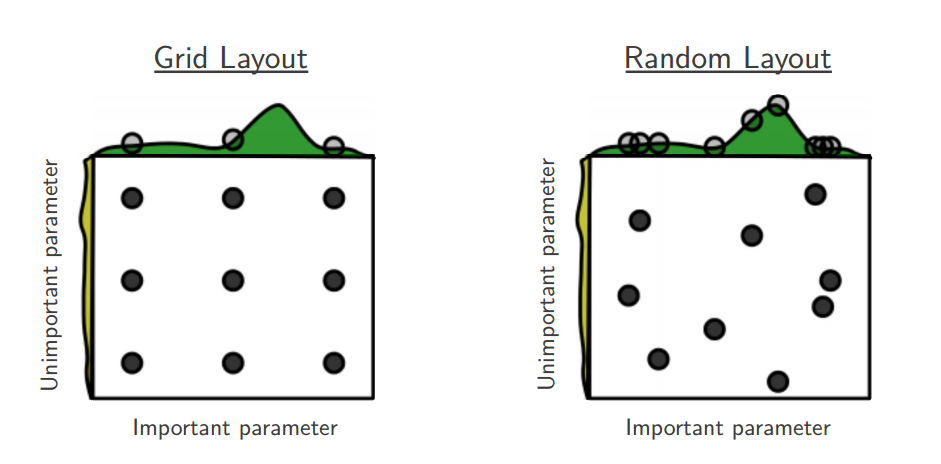
\includegraphics[width=\textwidth]{images/random_search.png}
\end{figure}
\pause
\vfill
In any case, you need to know upper/lower bounds on the parameters
\end{frame}

\begin{frame}{Conclusion}
There are several ways to evaluate a model depending on
\begin{itemize}
	\item \textbf{What you value} in your application
	\begin{itemize}
		\item Proper metric \& loss function choices
	\end{itemize}
	\item \textbf{Your data}
	\begin{itemize}
		\item Proper evaluation framework choice
	\end{itemize}
\end{itemize}
\vfill
\pause
Think about this before applying a \textbf{random algorithm} and evaluating it with a \textbf{random metric}!
\end{frame}

\begin{frame}
	\center
	\huge{Thank you! Questions?}
\end{frame}

\end{document}